\subsection{Funkcinis-reaktyvus programavimas}

\subsubsection{Įvadas}

Anot \cite{Survey}, funkcinis-reaktyvus programavimas, toliau dažnai vadinamas tiesiog FRP, yra būdas modeliuoti reaktyvų - besikeičiančius laiko tekmėje bei reaguojančius į išorinį stimulą - elgesį visiškai funkcinėse programavimo kalbose. FRP leidžia deklaratyviu ir paprastu būdu modeliuoti sistemas, kurios turi reaguoti į duomenis bėgant laikui.

\subsubsection{Pagrindinis tikslas}

Pagrindinis funkcinio-reaktyvaus programavimo tikslas \cite{Survey}:

\begin{itemize}

	\item saugus programavimas - kompiliatorius turi kiek įmanoma patikrinti programų korektiškumą;

	\item efektyvus programavimas - programos turėtų veikti realiu laiku, todėl efektyvios ir optimizuotos operacijos yra būtinos;

	\item komponavimas - FRP leidžia kurti programas iš smulkesnių programų, o ne orientuotą į problemą, vientisą kodą.

\end{itemize}

\subsubsection{Sąvokos}

Pagrindinės FRP sąvokos yra:

\begin{itemize}

	\item signalai arba elgsena - besikeičiančios laike reikšmės;

	\item įvykiai - kolekcija momentinių reikšmių arba laiko-reikšmės poros.

\end{itemize}

FRP pasiekia reaktyvumą naudodamas konstrukcijas, kurios tiksliai apibrėžia kaip signalai arba elgsena pasikeičia reaguodami į įvykius. Tai yra pagrindinis būdas išreiškiant bei realizuojant elgseną. Kitu būdu, elgsena gali būti laiko semantinės funkcijos\footnote{http://msdl.cs.mcgill.ca/people/tfeng/docs/as/node5.html}, kuriose laikas yra pakeičiamas kilus įvykiui \cite{Nilsson:2002:FRP:581690.581695}.

\subsubsection{Sąvybės}

Anot anksčiausios funkcinio-reaktyvaus programavimo formuluotės \cite{ElliottHudak97:Fran}, pagrindinės sąvybės, kuriomis pasižymi FRP:

\begin{itemize}

	\item elgsenos arba signalų modeliavimas bėgant laikui,

	\item įvykių, kurie turi baigtinį skaičių atsitikimų daugelyje laiko taškų, modeliavimas,

	\item perjungimas (angl. switching) - sistema gali pasikeisti dėl atsitikusių įvykių,

	\item analizės detalių, tokių kaip reaktyvaus modelio įvykių ėmimo dažnis, atskyrimas.

\end{itemize}

\subsubsection{Įvykių srautas}

Pagal \cite{Bass:2007:Mythbusters}, įvykių srautas yra eilė pagal laiką surikiuotų įvykių, pavyzdžiui akcijų rinkos srautas.

Įvykių srautas kaip duomenų srauto tipas formaliai atrodo kaip pora (s, t), kur s yra seka surikiuotų sąrašo įvykių, o t yra seka laiko intervalų ir kiekvienas intervalas yra netuščias.

Tokio duomenų srauto pavyzdžiai gali būti:

\begin{itemize}

	\item akcijų kursas,

	\item paspaudimų srautas,

	\item tinklo srautas,

	\item GPS\footnote{http://en.wikipedia.org/wiki/Global\_Positioning\_System} duomenys.

\end{itemize}

Įvykių srauto apdorojimas pagal atsitikimo laiką turi privalumų:

\begin{itemize}

	\item įvykių apdorojimo algoritmai naudoja mažai atminties, nes jiems nereikia prisiminti daug įvykių;

	\item algoritmai gali būti labai greiti;

	\item gavus įvykį, skaičiavimai atliekami iškart, todėl galima perduoti rezultatą kitam skaičiavimui ir pamiršti įvykį.

\end{itemize}

Įvykių srauto apdorojimas labiau akcentuoja didelio našumo duomenų gavimą ir matematinių algoritmų pritaikymą įvykių duomenims. Taip pat įvykių srautai įprastai pritaikomi konkrečiai sistemai ar organizacijai.

\subsubsection{Įvykių srautas funkciniame programavime}

Vietoje įvykių srauto, galima naudoti klausytojo projektavimo šabloną \cite{WhiteboardPattern}, tačiau ilgame programinės įrangos kūrimo gyvavimo cikle įvykių srauto naudojimas palengvina kai kuriuos dalykus. Pavyzdžiui, imperatyvaus programavimo atžvilgiu, viename metode turime klausytoją, kuris reaguoją į situaciją \textit{A}, tačiau iškilus situacijai \textit{B}, šis klausytojas yra pašalinamas. Šiuo atveju programinis kodas, kuris valdo klausytojo gyvavimo ciklą yra įsipynęs keliose skirtingose kodo vietose, ko pasekoje tai reiškia, jog yra sunkiau palaikyti, stebėti, keisti bei suprasti šias vietas. Įvykių srautas yra pirmosios klasės reikšmės, todėl jį galima abstrahuoti \cite{EPFL-REPORT-176887}. Abstrahuojant klausytojų gyvavimo ciklo valdymo idėją tampa lengviau programuoti pagal tai kas turėtų nutikti, o ne pagal tai, ką kompiuteris turėtų daryti toliau. Tačiau turbūt didesnis įvykių srauto pranašumas yra tai, jog pastarasis gali būti transformuojamas ir komponuojamas. Toliau bus aprašomi operacijos arba veiksmai bei sutrumpinti išeities kodo pavyzdžiai, kuriuos galima atlikti su įvykių srautu remiantis Reactive Web\footnote{http://scalareactive.org} karkasu, skirtu Scala\footnote{http://www.scala-lang.org} programavimo kalbai.

Pirmas veiksmas - įvykio srauto sukūrimas. Jis pavaizduotas \ref{creation} kodo pavyzdyje.  Pirmiausia sukuriamas įvykių šaltinis, kuris po to priskiriamas įvykių srautui.

\begin{lstlisting}[caption=- įvykių srauto sukūrimas, label=creation]
	val eventSource = new EventSource[String]{}
	scheduleTask(10000) {
		eventSource.fire("Event after 10 seconds")
	}

	val eventStream: EventStream[String] = eventSource
\end{lstlisting}

Taip pat \textit{EventSource} (įvykių šaltinis) turi naudingą poklasį \textit{Timer} (laikrodis). Jo realizacija pavaizduota \ref{timer} kodo pavyzdyje. Šis sukuria tiksėjimo įvykius duotu laiko intervalu.

\begin{lstlisting}[caption=- įvykių srauto sukūrimas, label=timer]
	val timer = new Timer(0, 2000, {t =>  t >= 32000})

	for(t <- timer)
    	yield "timer: " + t.toString
\end{lstlisting}

Įvykių srautas valdo kolekciją klausytojų, tačiau konceptualiai reikėtų mąstyti kitaip. Klausytojo pridėjimas iš tikrųjų reiškia funkcijos iškvietimą kiekvienam kilusiui įvykiui, kitais žodžiais kiekvienam įvykių srauto įvykiui. Lygiai taip pat kaip Scala programavimo kalboje norint įvykdyti funkciją kiekvienai kolekcijos reikšmei yra iškviečiama \textit{foreach} funkcija. Tačiau įvykių srauto atveju, \textit{foreach} grąžina rezultatą akimirksniu, o funkcija yra išsaugoma ir vėliau įvykdoma kai tik iššaunamas koks nors įvykis. Šio atvejo praktinis variantas pademonstruotas \ref{foreach} kodo pavyzdyje.

\begin{lstlisting}[caption=- klausytojų pridėjimas, label=foreach]
	val eventSource = new EventSource[String] {}
	  
	// The following is syntactic sugar for
	// eventSource.foreach(event => alert("You fired: '" + event + "'"))
	for(event <- eventSource) {
	 	alert("You fired: '" + event + "'")
	}

\end{lstlisting}

Rinkinys transformacijos metodų įvykių srautą padaro labai universaliu. Šios transformacijos grąžina modifikuotą įvykių srautą. Transformacijas galima atlikti viena po kitos. Tai primena transformacijas galimas su Scala kolekcijomis, pavyzdžiui \ref{collectionTransformation} kodo pavyzdyje. Kai tik originalus įvykių srautas gauna įvykį, transformuotas įvykių srautas iššauna savo įvykį pritaikant klausytojo funkciją.

\begin{lstlisting}[caption=- kolekcijos transformacijos, label=collectionTransformation]
	List(1,2,3).map(_ * 10).filter(_ < 25)
\end{lstlisting}

Jeigu įvykių srautas gauna labai daug įvykių, tačiau aktualūs yra tik dalis jų, galima naudoti filtravimą, tai yra \textit{filter} metodą. Tai demonstruojama \ref{filter} kodo pavyzdyje. Čia kiekvienam įvykiui yra pritaikomas predikatas. Jeigu jis įvertinimas kaip teisingas arba kitaip \textit{true}, įvykis yra iššaunamas transformuotame įvykių sraute.

\begin{lstlisting}[caption=- įvykių srauto filtravimas, label=filter]
	val eventSource = new EventSource[String] {}
	eventSource.filter(_.length < 5)
\end{lstlisting}

Kitas esminis kolekcijų metodas yra \textit{map}. Jis leidžia transformuoti kolekciją pritaikant tam tikrą funkciją kiekvienam kolekcijos elementui. Pritaikius yra grąžinama nauja modifikuota kolekcija. Lygiai taip pat šis metodas gali būti pritaikytas įvykių srautui. Šis atvejis demonstruojamas \ref{map} kodo pavyzdyje. 

\begin{lstlisting}[caption=- įvykių visiškas transformavimas, label=map]
	val eventSource = new EventSource[String] {}
	eventSource.map(_.reverse)
\end{lstlisting}


Įvykių srautam taip pat galima pritaikyti \textit{flatmap} metodą. Scala kolekcijose šis metodas pritaiko funkciją visiems elementams, kuri grąžina naują kolekciją, kurioje sujungiamos visos grąžintų kolekcijų reikšmės. Pavyzdys pateiktas kodo pavyzdyje \ref{collectionsFlatmap}. Operacijos \textit{map} atveju būtų grąžinta reikšmė \textit{List(List(10, 11, 12), List(20, 21, 22), List(30, 31, 32))}, tačiau operacija \textit{flatMap} sujungia grąžintų kolekcijų reikšmes. 

\begin{lstlisting}[caption=- flatmap Scala kolekcijose, label=collectionsFlatmap]
	val original = List(1, 2, 3)
	val flatMapped = original.flatMap(x => List(x*10,x*10+1,x*10_2))
	flatMapped == List(10,11,12,  20,21,22,  30,31,32) 
\end{lstlisting}

Panašiai veikia \textit{flatMap} metodas įvykių srautuose. Pastarasis leidžia sukurti įvykių srautą, kuris iššauna įvykius, kurie yra iššauti kitų įvykių srautų. Metodas demonstruojamas \ref{flatmap} kodo pavyzdyje. Čia figūra yra išplečiama, o po to išnyksta.

\begin{lstlisting}[caption=- flatmap įvykių sraute, label=flatmap]
	// Assuming Shape is a case class with scale and opacity values
	// and millisTimer fires events once per millisecond, starting
	// at zero.
	// Scale should animate from 0 to 1 over the first second,
	// and opacity should animate from 1 to 0 over the next.
	def compositeAnimation(millisTimer: EventStream[Long], shape: Shape): EventStream[Shape] = {
	  val scale: EventStream[Double] =
	    millisTimer.map(m => m/1000.0)
	  val opacity: EventStream[Double] =
	    millisTimer.map(m => 1 - (m-1000)/1000.0)
	  val seconds = millisTimer.filter(_ % 1000 == 0).map(_ / 1000).
	    takeWhile(_ < 2000)
	  
	  seconds.flatMap {
	    case 0 => scale
	    case 1 => opacity
	  }
	}
\end{lstlisting}

Imperatyviose kalbose, dažna užduotis yra iteruoti per masyvą ir atlikti tam tikrus veiksmus. Šiam veiksmui atlikti naudojamas tam tikras skaičius kintamųjų veiksmam atlikti, pavyzdžiui skaičiavimam. Funkciniame programavime šiam tikslui dažnai yra naudojamas \textit{foldLeft} metodas. Pastarasis priima pradinę reikšmę arba kitaip būseną ir funkciją, kuri priima paskutinę reikšmę arba būseną ir kitą kolekcijos elementą. Kiekvienam elementui funkcija grąžina reikšmę arba būseną, kuri naudojama sekančiam funkcijos kvietimui. Verta pastebėti, jog funkcinis programavimas čia leidžia kodą vykdyti lygiagrečiai jo visiškai nekeičiant. \ref{collectionsFoldLeft} kodo pavyzdys demonstruoja sąrašo elementų sumos skaičiavimą.

\begin{lstlisting}[caption=- sąrašo elementų skaičiavimas naudojant flatmap, label=collectionsFoldLeft]
	list.foldLeft(0){(totalSoFar, nextElement) => totalSoFar + nextElement}
	//more commonly written as list.foldLeft(0)(_ + _)
\end{lstlisting}

Panašiai \textit{foldleft} metodą galima pritaikyti įvykių srautam. Demonstracija \ref{foldleft} kodo pavyzdyje.

\begin{lstlisting}[caption=- foldleft metodas įvykių sraute, label=foldleft]
	case class AvgState(total: Double, count: Int)
	val eventSource = new EventSource[String] {}
	
	eventSource.foldLeft(AvgState(0,0)){
      case (AvgState(total, count), s) => AvgState(total+s.length,count+1)
    } map {
      case AvgState(total, count) =>
        "Average length so far: " + (total/count)
    }
\end{lstlisting}

Įvykių srautus galima ne tik transformuoti, bet ir komponuoti, tai yra sujungti. Demonstracija \ref{merge} kodo pavyzdyje. Įvykių srautas \textit{allClicks} iššauna įvykį kai bet kuris iš kitų įvykių srautų iššauna įvykį.

\begin{lstlisting}[caption=- įvykių srautų sujungimas, label=merge]
	val allClicks = leftClicks | middleClicks | rightClicks
\end{lstlisting}

Įvykių srautas atvaizduoja įvykius kaip srautą diskrečių reikšmių laiko tekmėje, taigi šios reikšmės egzistuoja momentiškai. Tačiau įvykių srautą taip pat galima paversti signalu. Signalas atvaizduoja besitęsiančią reikšmę, tai yra turi dabartinę reikšmę. Kai signalo reikšmė pasikeičia, įvykių srautas iššauna naują įvykį. Įvykių srautą norint paversti signalu galima naudoti \textit{hold} metodą, kuriam yra paduodama pradinė reikšmė. Demonstracija \ref{hold} kodo pavyzdyje.

\begin{lstlisting}[caption=- įvykių srautų pavertimas signalu, label=hold]
	val eventSource = new EventSource[String] {}
  	val signal = eventSource.hold("(initial value of signal)")
  
  	def render = Demos.eventSourceInput(eventSource) ++
    	<p>Signal value: '{Demos.signalOutput(signal)}'</p>
\end{lstlisting}

\subsection{Įvykių kaupimas}

Šiame skyriuje yra aprašomos žinios apie įvykių kaupimą, pliusus ir minusus, įvykių srautus bei įvykių kaupimą funkciniame programavime remiantis daugiausia Vaughn Vernon surinkta ir aprašyta informacija \cite{vernon2013implementing}.

\subsubsection{Įvadas}

Kartais verslui svarbu fiksuoti objekto pasikeitimus domeno modelyje\footnote{http://en.wikipedia.org/wiki/Domain\_model}. Šiuos pasikeitimus galima stebėti skirtingais būdais. Įprastai yra pasirenkama stebėti kai esybė\footnote{http://en.wikipedia.org/wiki/Entity} yra:

\begin{itemize}

	\item sukurta,

	\item paskutinį kartą modifikuota

	\item bei kas atliko modifikaciją.

\end{itemize}

Tačiau šis būdas nepateikia jokios informacijos apie vienkartinius pasikeitimus.

Atsiradus poreikiui stebėti pasikeitimus detaliau, verslas reikalauja dar daugiau metaduomenenų\footnote{http://en.wikipedia.org/wiki/Metadata}, ko pasekoje tokie faktai kaip individualios operacijos laiko tekmėje bei jų įvykdymo laikas tampa svarbūs. Šie poreikiai verčia įvesti audito žurnalą fiksuoti labai tikslias panaudojimo atvejų metrikas, tačiau pastarasis būdas turi apribojimų. Jis gali atskleisti dalį informacijos apie tai kas nutiko sistemoje, leisti rasti bei ištaisyti dalį riktų bei klaidų programinėje įrangoje. Bet audito žurnalas neleidžia patikrinti domeno objekto būsenos prieš ir po tam tikrų pasikeitimų. O jeigu būtų galima išgauti daugiau informacijos iš pasikeitimų stebėjimo?

Visi programinės įrangos kūrėjai susiduria su labai tiksliu pasikeitimų stebėjimu. Įprastas ir populiarus pavyzdys yra išeities kodo saugyklos, tokios kaip CVS\footnote{http://www.nongnu.org/cvs/}, Subversion\footnote{http://subversion.apache.org/}, Git\footnote{http://git-scm.com/} arba Mercurial\footnote{http://mercurial.selenic.com/}. Visos šios pataisų valdymo sistemos leidžia stebėti pirminių failų pasikeitimus. Įrankiai leidžia peržiūrėti išeities kodo artefaktus nuo pačios pirmosios pataisos iki paskutinės. Kai visi išeities failai yra nusiunčiami į pataisų kontrolės sistemą, ši gali stebėti pasikeitimus viso programinės įrangos kūrimo gyvavimo ciklo metu.

Jeigu šis principas būtų pritaikytas vienai esybei, tada vienam agregatui\footnote{http://martinfowler.com/bliki/DDD\_Aggregate.html} bei galiausiai kiekvienam modelio agregatui, galima suprasti kokią naudą atneša sistemos objektų pasikeitimų stebėjimas:

\begin{itemize}

	\item Kas būtent nutiko modelyje, jog agregato egzempliorius buvo sukurtas?

	\item Kas nutiko agregato egzemplioriui bėgant laikui? (Operacijų požiūriu)

\end{itemize}

Turint visų atliktų operacijų istoriją, galima palaikyti laikinus modelius. Toks kaitos stebėjimas yra įvykių kaupimo principas. \ref{pic:es} diagramoje pateika šio principo aukšto lygio reprezentacija. Agregatai publikuoja įvykius, kurie yra išsaugomi įvykių saugykloje ir naudojami sekti modelio būsenos pasikeitimus. Verta paminėti, jog įvykiai reprezentuoja tam tikrą būsenos pasikeitimą bėgant laikui, todėl jie nėra atnaujinami arba ištrinami. Saugykla nuskaito įvykius iš įvykių saugyklos ir pritaiko juos vieną po kito taip atkurdama agregato būseną. 

\begin{figure}[ht]
	\centering
	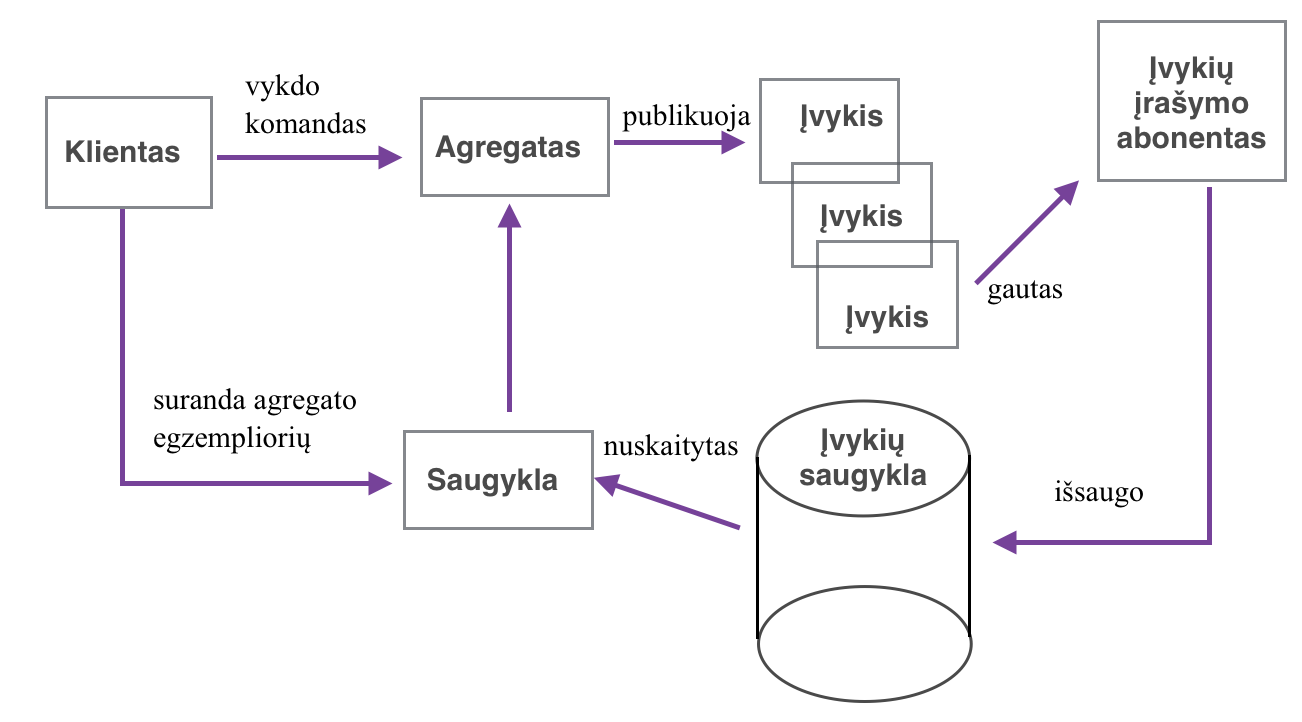
\includegraphics[width=0.9\linewidth]{pics/es.png}
	\caption{Įvykių kaupimo aukšo lygio reprezentacija}
	\label{pic:es}
\end{figure}

\subsubsection{Momentinė kopija}

Ilgame periode sistemoje susikaupia daugybė įvykių. Atkuriant agregato būseną reikia atkartoti šimtus, tūkstančius ar net milijonus įvykių. Tai tampa šio modelio silpnąja puse, nes įvykių atkartojimas užtrunka vis ilgiau sistemai plečiantis.

Tačiau šio duomenų kamsčio galima išvengti naudojant agregato būsenos momentines kopijas. Tam tikrame įvykių saugyklos istorijos taške yra padaroma agregato būsenos kopija. Serializuota agregato būsena yra įrašoma į įvykių saugyklą. Nuo to momento, agregatas yra atkuriamas pirmiausia naudojantis naujausia jo būsenos momentine kopija ir tik po to atkartojami visi naujesni įvykiai.

Momentinės kopijos nėra atkuriamos atsitiktinai. Jos gali būti kuriamos kas apibrėžtą skaičių įvykių. Šis skaičius turėtų būti parinktas analizuojant domeno sritį bei sistemą ir radus optimalų variantą. Tikėtinai gali būti 50 arba 100 įvykių tarp momentinių kopijų.

\subsubsection{Įvykių kaupimo privalumai ir trūkumai}

Kaip saugojimo mechanizmas, įvykių kaupimas stipriai skiriasi ir pakeičia ORM\footnote{http://www.orm.net/} įrankį. Kadangi įvykiai dažnai įrašomi kaip dvejetainės reprezentacijos, jie negali būti optimaliai naudojami užklausoms atlikti. Faktiškai įvykių kaupimu pagrįstoms saugykloms tereikia vienos operacijos - gauti įrašus pagal unikalią agregato tapatybę \cite{CQRS:GregYoung}. To pasekoje užklausom daryti reikia kito kelio. Dažniausiai tam pasirenkamas CQRS\footnote{http://martinfowler.com/bliki/CQRS.html} principas \cite{Betts:2013:ECE:2509680}. 

Įvykių kaupimas verčia kitaip mąstyti apie domeno modelį. Įvykių istorija gali padėti surasti bei ištaisyti sistemos defektus bei klaidas \cite{SeanFitz2012}. Derinimas naudojant istoriją visų veiksmų, kurie nutiko sistemoje, turi didžiulį pranašumą. Įvykių kaupimas gali vesti prie didelio našumo domeno modelių, tai yra palaikyti ypač didelį skaičių operacijų per sekundę. Pavyzdžiui, įrašymas į vieną duomenų saugyklos lentelę yra ypač greitas. Negana to, tai leidžia CQRS užklausų modelį išplėsti horizontaliai, nes duomenų šaltinio atnaujinimai įvykdomi fone, kai įvykių saugykla yra atnaujinama naujais įvykiais.

\subsubsection{Įvykių kaupimas funkciniame programavime}

Vaughn Vernon pateikia keletą pastebėjimų apie įvykių kaupimą funkciniame programavime, kurie gali būti naudingi atliekant projektinius sprendimus bei eksperimentinį tyrimą:

\begin{itemize}

	\item Agregatas projektuojamas kaip nekintantis būsenos įrašas kartu su funkcijomis, kurios keičia būseną. Šios funkcijos paprasčiausiai priima būsenos įrašą ir įvykių argumentus ir gražina naują būsenos įrašą kaip rezultatą. Tokia funkcija pavaizduota \ref{aggregate} kodo pavyzdyje.

\begin{lstlisting}[caption=- agregato būsenos keitimas, label=aggregate]

	Funkcija<Busena, Ivykis, Busena>

\end{lstlisting}

	\item Dabartinė agregato būsena gali būti apibrėžta kaip suskleidimas į kairę visų praeities įvykių, kurie yra perduodami būseną keičiančiai funkcijai.

	\item Agregato metodai gali būti išreikšti kaip kolekcija funkcijų be būsenos.

	\item Įvykių saugykla gali būti suvokiama bei naudojama kaip funkcinė duomenų bazė, nes ji perduoda argumentus funkcijoms, kurios keičia agregato būseną. Momentinės kopijos įvykių saugykloje primena įsiminimą atmintyje\footnote{http://en.wikipedia.org/wiki/Memoization} funkciniame programavime.

\end{itemize}

\subsection{Monados}

\subsubsection{Terminas}

Funkciniame programavime monada yra struktūra, kuri atspindi skaičiavimus, apibrėžtus kaip seka žingsnių. Tipas kartu su monados struktūra apibrėžia ką reiškia vykdyti operacijas viena po kitos bei naudoti to pačio tipo įdėtines funkcijas. Tai leidžia kurti komandų grandines, kurios pažingsniui apdoroja informaciją, kur kiekvienas veiksmas yra dekoruojamas naujomis apdorojimo taisyklėmis, kurias apibrėžia monada \cite{OSullivan:2008:RWH:1523280}. Taip pat monada gali būti laikoma kaip funkcinis projektavimo šablonas, skirtas kurti daugybinius tipus \cite{monadicDesign}.

\subsubsection{Taisyklės}

Anot \cite{Wadler:1995:MFP:647698.734146}, monadų operacijos turi tenkinti tris taisykles:

\begin{itemize}

	\item Kairiojo vienetotapatybės (angl. left unit/identity) - suskaičiuojama reikšmė \textit{a}, rezultatui priskiriamas \textit{b} ir suskaičiujama \textit{n} reikšmė. Rezultatas yra toks pat kaip \textit{n} kai \textit{a} reikšmė pakeičiama \textit{b} reikšme. Parodyta \ref{pic:left} paveikslėlio formulėje.

\begin{figure}[ht]
	\centering
	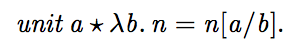
\includegraphics{pics/left.png}
	\caption{Perkėlimo į kairę taisyklė}
	\label{pic:left}
\end{figure}

	\item dešiniojo vieneto/tapatybės (angl. right unit/identity) - suskaičiuojama reikšmė \textit{m}, rezultatas priskiriamas \textit{a} ir grąžinama \textit{a}. Rezultatas yra toks pat kaip \textit{m}. Parodyta \ref{pic:right} paveikslėlio formulėje.

\begin{figure}[ht]
	\centering
	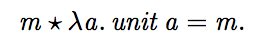
\includegraphics{pics/right.png}
	\caption{Perkėlimo į dešinę taisyklė}
	\label{pic:right}
\end{figure}

	\item Asociatyvumas - suskaičiuojama reikšmė \textit{m}, rezultatas priskiriamas \textit{a}, suskaičiuojamas \textit{n}, rezultatas priskiriamas \textit{b}, suskaičiuojama \textit{o}. Skliaustelių padėtis šiuo atveju yra nesvarbi. Kintamojo \textit{a} apimtis įtraukia \textit{o} kairėje, tačiau neįtraukia \textit{o} dešinėje, todėl ši taisyklė galioja tik tada kai \textit{a} nėra laisvas nuo \textit{o}. Parodyta \ref{pic:associative} paveikslėlio formulėje.

\begin{figure}[ht]
	\centering
	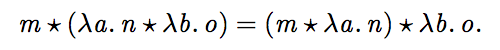
\includegraphics{pics/associative.png}
	\caption{Asociatyvumas}
	\label{pic:associative}
\end{figure}

\end{itemize}

\subsubsection{Tolesnis darbas}

Kitame mokslinio tyrimo etape ruošiamąsi įrodyti, kad funkcinį-reaktyvų programavimą įmanoma taikyti įvykių kaupimo sistemose. Šiam tikslui pasiekti toliau bus nagrinėjamos monados, jų komponavimo būdai. Kad geriau suprasti monadas turbūt prireiks įgauti žinių kategorijų teorijoje, daugiau žinių apie funkcinį programavimą, pavyzdžiui tipizuotos klasės, parametrizuoti tipai ir t.t.

\subsection{Išvados}

Literatūros analizės metu remiantis kitų autorių patirtimi:

\begin{itemize}

\item išnagrinėtas funkcinis-reaktyvus programavimas,

\item išnagrinėtas įvykių kaupimo principas,

\item išnagrinėti įvykių srautai bei operacijos su jais,

\item susipažinta su įvykių kaupimu funkciniame programavime,

\item susipažinta su monadomis,

\item įvaldyta sąvokų sistema, susijusi su nagrinėjama tematika.

\end{itemize}
